\documentclass{beamer}


\usepackage{amsmath}
\usepackage[style=alphabetic,url=true]{biblatex}
\usepackage{environ}
\usepackage{geometry}
\usepackage{graphicx}
\usepackage{tikz}
\usepackage[T2A]{fontenc}
\usepackage[utf8]{inputenc}
\usepackage[cache=false]{minted}
\usepackage{amsmath}
\usepackage{amsfonts}
\usepackage{amssymb}
\usepackage{calrsfs}
\usepackage{animate}
\usepackage{xmpmulti}


% \usetheme{Bergen}

\usecolortheme{beaver}

\setbeamertemplate{itemize item}[circle]
\setbeamertemplate{itemize subitem}{--}
\addtobeamertemplate{navigation symbols}{}{
  \usebeamerfont{footline}%
  \usebeamercolor[fg]{footline}%
  \hspace{1em}%
  \insertframenumber/\inserttotalframenumber
}
\graphicspath{ {./graphics/} }
\setminted[Python]{
  fontsize=\tiny
}
\BeforeBeginEnvironment{minted}{\medskip}
\AfterEndEnvironment{minted}{\medskip}
\usetikzlibrary{matrix}
\tikzset{
  stack/.style={
    matrix of nodes,
    nodes={
      fill=lightgray,draw,text=black,font=\sffamily\bfseries,
      text height=11pt,text depth=3pt,baseline=center, minimum width=1cm
    },
    column sep=-\pgflinewidth/2
  }
}

\title{
  Bitcoin and Cryptocurrency Technologies \\
  Lecture 8: Bitcoin Wallets
}

\author{Yuri Zhykin}
\date{Apr 19, 2021}

\begin{document}

\frame{\titlepage}

\begin{frame}
  \frametitle{UTXO Set}
  \begin{itemize}
  \item All bitcoin in existence is represented by a \textbf{UTXO set} - a set
    of all unspent transaction outputs.
  \item Every ``coin'' consists of the amount of \textbf{satoshis} and the
    corresponding lock script.
  \item In order to verify the received transaction, a Bitcoin user checks that
    transaction is correctly constructed and if the outputs used by the
    transaction are included in the \textbf{UTXO set}.
  \item Whole Bitcoin protocol works to ensure the \textbf{consistency} of of
    the \textbf{UTXO set}.
  \end{itemize}
\end{frame}

\begin{frame}
  \frametitle{Bitcoin Ownership}
  \begin{itemize}
  \item \textbf{Owning bitcoin} means that some entity can provide the correct
    \textbf{unlock script} to the \textbf{lock script} of some of the outputs in
    \textbf{UTXO set}.
  \item Lock scripts are visible publicly, so ideally every ``piece'' of bitcoin
    should have a different lock script.
  \item Otherwise, it is immediately visible how much bitcoin a certain entity
    owns.
  \item Any software, hardware or object that stores data needed to construct
    unlock scripts is technically a \textbf{Bitcoin wallet}.
    
  \end{itemize}
\end{frame}

\begin{frame}
  \frametitle{Standard Lock Scripts}
  \begin{itemize}
  \item \textbf{P2PK} - Pay to Public Key
    \break
    \begin{tabular}{rl}
      &\tiny\mintinline[bgcolor=lightgray]{Lisp}{<pubKey> OP_CHECKSIG;} \\
    \end{tabular}
  \item \textbf{P2MS} - Pay to Multi-Signature
    \break
    \begin{tabular}{rl}
      &\tiny\mintinline[bgcolor=lightgray]{Lisp}{<M> <pk1> ... <pkN> <N> OP_CHECKMULTISIG;} \\
    \end{tabular}
  \item \textbf{P2PKH} - Pay to Public Key Hash
    \break
    \begin{tabular}{rl}
      &\tiny\mintinline[bgcolor=lightgray]{Lisp}{OP_DUP OP_HASH160 <pubKeyHash> OP_EQUALVERIFY OP_CHECKSIG;} \\
    \end{tabular}
  \item \textbf{P2SH} - Pay to Script Hash
    \break
    \begin{tabular}{rl}
      &\tiny\mintinline[bgcolor=lightgray]{Lisp}{OP_HASH160 <scriptHash> OP_EQUAL;} \\
    \end{tabular}
  \item \textbf{P2WPKH} - Pay to \textbf{Witness} Public Key Hash
    \break
    \begin{tabular}{rl}
      &\tiny\mintinline[bgcolor=lightgray]{Lisp}{OP_0 <20-byte-witness-data>;} \\
    \end{tabular}
  \item \textbf{P2WSH} - Pay to \textbf{Witness} Script Hash
    \break
    \begin{tabular}{rl}
      &\tiny\mintinline[bgcolor=lightgray]{Lisp}{OP_0 <32-byte-witness-data>;} \\
    \end{tabular}
  \end{itemize}
\end{frame}

\begin{frame}
  \frametitle{Segregated Witness}
  \begin{itemize}
  \item Softfork in the network, activated on 24 August 2017.
  \item Proposed in a series of \textbf{Bitcoin Improvement Proposals} -
    BIP-0141, BIP-0143, BIP-0144 and BIP-0148.
  \item Main idea is to move the large unlock scripts out of the transaction
    data that is included in the blocks.
  \end{itemize}
\end{frame}

\begin{frame}
  \frametitle{Bitcoin Addresses 1/3}
  \begin{itemize}
  \item Bitcoin uses several human-oriented encodings to encode addresses and
    keys:
    \begin{itemize}
    \item \textbf{Base58Check}
      \break
      \begin{tabular}{rl}
        &${\scriptstyle \mathit{Base58Check}(t, data) = \mathit{Base58}(t + data + \mathit{HASH256}(t + data)[0:4])}$ \\
      \end{tabular}
      \break
      where \textit{Base58}
      \break
      \begin{tabular}{rl}
        &${\scriptstyle 123456789ABCDEFGHJKLMNPQRSTUVWXYZabcdefghijkmnopqrstuvwxyz}$ \\
      \end{tabular}
    \item \textbf{Bech32}
      \break
      \begin{tabular}{rl}
        &${\scriptstyle \mathit{Bech32}(t, data) = t + "1" + \mathit{Base32'}(data +
          \mathit{Bech32Checksum}(t, data))}$ \\
      \end{tabular}
      where \textit{Base32'}
      \break
      \begin{tabular}{rl}
        &${\scriptstyle qpzry9x8gf2tvdw0s3jn54khce6mua7l}$ \\
      \end{tabular}
    \end{itemize}
  \end{itemize}
\end{frame}

\begin{frame}
  \frametitle{Bitcoin Addresses 2/3}
  \begin{itemize}
  \item \textbf{P2PK} and \textbf{P2MS} do not have defined address formats.
  \item \textbf{P2PKH} address format is defined as follows
    \break
    \begin{tabular}{rl}
      &\tiny\mintinline[bgcolor=lightgray]{Lisp}{OP_DUP OP_HASH160 <pubKeyHash>
        OP_EQUALVERIFY OP_CHECKSIG;} \\
      &${\scriptstyle A_{\mathit{p2pkh}} = \mathit{Base58Check}(0x00 +
        pubKeyHash)}$ \\
      &{\scriptsize \quad\quad\quad \textbf{1}7VZNX1SN5NtKa8UQFxwQbFeFc3iqRYhem} \\
      &${\scriptstyle A'_{\mathit{p2pkh}} = \mathit{Base58Check}(0x6F +
        pubKeyHash)}$ \\
      &{\scriptsize \quad\quad\quad \textbf{m}ipcBbFg9gMiCh81Kj8tqqdgoZub1ZJRfn} \\
    \end{tabular}
  \item \textbf{P2SH} address format is defined as follows
    \break
    \begin{tabular}{rl}
      &\tiny\mintinline[bgcolor=lightgray]{Lisp}{OP_HASH160 <scriptHash> OP_EQUAL;} \\
      &${\scriptstyle A_{\mathit{p2sh}} = \mathit{Base58Check}(0x05 +
        scriptHash)}$ \\
      &{\scriptsize \quad\quad\quad \textbf{3}EktnHQD7RiAE6uzMj2ZifT9YgRrkSgzQX} \\
      &${\scriptstyle A'_{\mathit{p2sh}} = \mathit{Base58Check}(0xC4 +
        scriptHash)}$ \\
      &{\scriptsize \quad\quad\quad \textbf{2}MzQwSSnBHWHqSAqtTVQ6v47XtaisrJa1Vc} \\
    \end{tabular}
  \end{itemize}
\end{frame}

\begin{frame}
  \frametitle{Bitcoin Addresses 3/3}
  \begin{itemize}
  \item \textbf{P2WPKH/P2WSH} address format is defined as follows
    \break
    \begin{tabular}{rl}
      &\tiny\mintinline[bgcolor=lightgray]{Lisp}{OP_0 <20-or-32-byte witnessData>;} \\
      &${\scriptstyle A_{\mathit{p2wpkh/p2wsh}} = \mathit{Bech32}("bc" +
        witnessVersion + witnessData)}$ \\
      &{\scriptsize \quad\quad\quad \textbf{bc1}qw508d6qejxtdg4y5r3zarvary0c5xw7k\textbf{v8f3t4}} \\
      &${\scriptstyle A'_{\mathit{p2wpkh/p2wsh}} = \mathit{Bech32}("tb" +
        witnessVersion + witnessData)}$ \\
      &{\scriptsize \quad\quad\quad \textbf{tb1}qw508d6qejxtdg4y5r3zarvary0c5xw7k\textbf{xpjzsx}} \\
    \end{tabular}
  \end{itemize}
\end{frame}

\begin{frame}
  \frametitle{Cryptographic Key Storage}
  \begin{itemize}
  \item All standard lock/unlock scripts are based on providing a signature
    matching the public key, whose hash is included in the script (either lock
    script, or unlock script in case of P2SH, P2WPKH and P2WSH).
  \item Since the form of the script is standardized, \textit{the only component
      that differs} is \textbf{the hash of the public key}.
  \item The only piece of data needed to construct a standard unlock script for
    the standard lock script is the \textit{corresponding private key}.
  \item All bitcoin wallets currently in use are simply \textbf{cryptographic
      key stores}:
    \begin{itemize}
    \item securely store private keys for owned ``coins'',
    \item generate new private keys/public keys/addresses,
    \item for every new block or transaction, verify if its lock script
      corresponds to a standard lock/unlock script that matches any of the
      stored keys (\textbf{optional}).
    \end{itemize}
  \end{itemize}
\end{frame}

\begin{frame}
  \frametitle{Simple Key Pool Wallets}
  \begin{itemize}
  \item Simplest Bitcoin wallet is a \textbf{single private key}.
  \item The address is included in the public chain data, so if
    \textbf{addresses are reused}, it is easy to calculate the amount of bitcoin
    owned by the same entity.
  \item Since \textit{reusing addresses} is bad, the solution is to simply
    generate a new key for every new incoming transaction.
  \item Wallet is just a file containing a list of keys for all ``coins'' owned.
  \item Backup is needed after every received transaction.
  \item The size of the key storage continues to grow and its unsafe to remove
    old keys as their addresses might still get used in the future.
  \end{itemize}
\end{frame}

\begin{frame}[fragile]
  \frametitle{Hierarchical Deterministic Wallets 1/2}
  \begin{itemize}
  \item \textbf{Hierarchical deterministic wallets} (\textbf{HD wallets}) were
    first introduced in 2011 and standardized by BIP-0032 in 2012.
  \item The core idea behind HD wallets is to generate a \textbf{master private
      key} and derive all future private keys from it.
  \item \textbf{Any private key in the hierarchy can be used to generate any child
      private keys}.
    \begin{tabular}{rl}
      &${\scriptstyle \mathit{CKD_{priv}}(k_{par}, c_{par}, i) = \mathit{HMACSHA512}(c_{par},
        k_{par}G||i) = I}$ \\
      &${\scriptstyle k_i = I[0:32] + k_{par} \pmod{n}}$ \\
      &${\scriptstyle c_i = I[32:64]}$ \\
    \end{tabular}
  \item \textbf{Any public key in the hierarchy can be used to generate any
      child public keys but not their private keys}.
    \begin{tabular}{rl}
      &${\scriptstyle \mathit{CKD_{pub}}(K_{par}, c_{par}, i) = \mathit{HMACSHA512}(c_{par},
        K_{par}||i) = I}$ \\
      &${\scriptstyle K_i = (I[0:32])G + K_{par} = (I[0:32] + k_{par})G = k_iG}$ \\
      &${\scriptstyle c_i = I[32:64]}$ \\
    \end{tabular}

  \end{itemize}
\end{frame}

\begin{frame}[fragile]
  \frametitle{Hierarchical Deterministic Wallets 2/2}
  \begin{itemize}
  \item BIP-0039 defines a way to encode the master key as a sequence of words.
  \item Most modern wallets show BIP-0039 \textbf{seed} on initialization.
  \item 2048 words in the dictionary.
  \item 12-word sequence contains 128 bits of security.
  \item Example:
\begin{minted}{text}
  fortune flush  weekend current
  key     hero   snake   leopard
  brisk   climb  timber  appear
\end{minted}
  \end{itemize}
\end{frame}

\begin{frame}
  \frametitle{Security: Mobile Wallets}
  \begin{itemize}
  \item Dozens of wallet applications exist for mobile devices (both iOS and
    Android):
    \begin{itemize}
    \item \textbf{BlueWallet} (iOS, Android, centralized server),
    \item \textbf{Green} (iOS, Android, centralized server),
    \item \textbf{Bitcoin Wallet} (Android, SPV node).
    \end{itemize}
  \item Main disadvantage of mobile wallets is that the keys are stored on a
    network-connected device, which is inherently insecure.
  \item Any security breach that allows attackers to access the data on the
    device may result in keys being stolen.
  \item OK to use for day-to-day transactions involving small amounts of
    bitcoin.
  \end{itemize}
\end{frame}

\begin{frame}[fragile]
  \frametitle{Security: Hardware Wallets}
  \begin{minipage}{0.6\textwidth}\raggedright
    \begin{itemize}
    \item Hardware wallets are dedicated \textbf{air-gapped} devices that
      specialized at generating and storing cryptographic keys:
      \begin{itemize}
      \item \textbf{Trezor Model T, Trezor One}
      \item \textbf{Ledger Nano S}
      \item \textbf{Coldcard}
      \item \textbf{BitBox02}
      \end{itemize}
    \end{itemize}
  \end{minipage}
  \begin{minipage}{0.3\textwidth}\raggedleft
    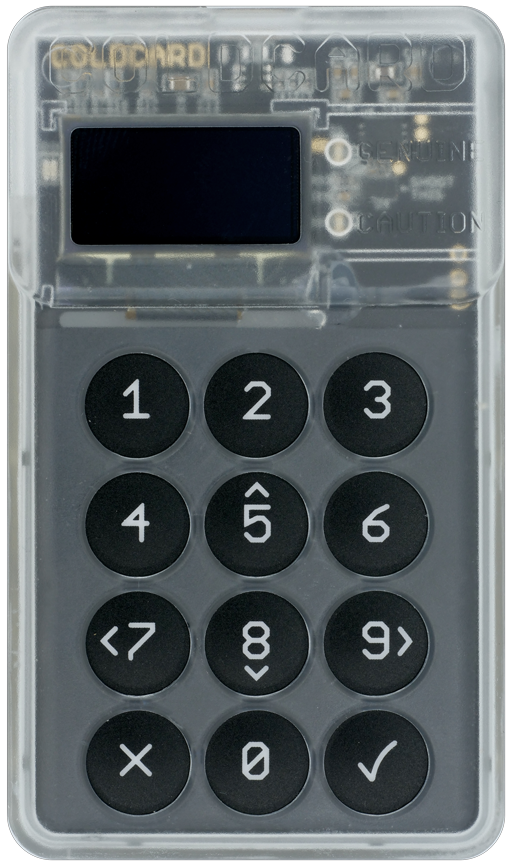
\includegraphics[width=0.7\linewidth]{coldcard-front}
  \end{minipage}
\end{frame}

\begin{frame}
  \frametitle{Security: Cold Storage}
  \begin{itemize}
  \item \textbf{Cold storage} is any method of storage that does not involve
    devices at all.
  \item HD seed can be written on a piece of paper and stored in a secure place,
    or even simply memorized.
  \item In order to use the bitcoin from cold storage, one needs to install the
    key on one a signing-capable device and only then create a transaction.
  \item \textbf{Resonably secure approach} to storing bitcoin:
    \begin{itemize}
    \item generate a new key with a dedicated hardware device (e.g. hardware
      wallet),
    \item create a cold backup of the \textbf{master private key} or seed,
    \item import the \textbf{master public key} to a device that will be used to
      track the storage,
    \item \textbf{delete the private key from the dedicated device}.
    \end{itemize}
  \end{itemize}
\end{frame}

\begin{frame}
  \frametitle{The End}
  \begin{center}
    Thank you!
  \end{center}
\end{frame}

\end{document}

%%% Local Variables:
%%% mode: latex
%%% TeX-master: t
%%% End:
